% 只是为了好玩
% 只是为了好玩.tex

\documentclass[12pt,UTF8]{ctexbook}

% 设置纸张信息。
\usepackage[a4paper,twoside]{geometry}
\geometry{
	left=25mm,
	right=25mm,
	bottom=25.4mm,
	bindingoffset=10mm
}

% 设置字体,并解决显示难检字问题。
\xeCJKsetup{AutoFallBack=true}
\setCJKmainfont{SimSun}[BoldFont=SimHei, ItalicFont=KaiTi, FallBack=SimSun-ExtB]

% 目录 chapter 级别加点(.)。
\usepackage{titletoc}
\titlecontents{chapter}[0pt]{\vspace{3mm}\bf\addvspace{2pt}\filright}{\contentspush{\thecontentslabel\hspace{0.8em}}}{}{\titlerule*[8pt]{.}\contentspage}

% 设置 part 和 chapter 标题格式。
\ctexset{
	part/name= {第,卷},
	part/number={\chinese{part}},
	chapter/name={第,篇},
	chapter/number={\chinese{chapter}}
}

% 图片相关设置。
\usepackage{graphicx}
\graphicspath{{Images/}}

% 设置署名格式。
\newenvironment{shuming}{\hfill\zihao{4}}

% 注脚每页重新编号,避免编号过大。
\usepackage[perpage]{footmisc}

\title{\heiti\zihao{0} 只是为了好玩}
\author{Linus Torvalds,David Diamond}
\date{}

\begin{document}

\maketitle
\tableofcontents

\frontmatter

\chapter{}



\mainmatter

\chapter{性爱体位}

性爱体位能够加深爱情与快感,是让彼此身体合拍最重要的技巧。

两人的身体在性爱中合不合拍,说穿了就是“确实刺激让对方舒服的性感带”,以及“阴茎与阴道无缝贴合”。

身体合拍可以说是达到欲仙欲死境界最重要的因素。或许你认为“性器官的大小或形状都是天生的,根本无可奈何”,其实没这回事。许多爱侣一开始身体未必合拍,却在“不知不觉中变成天造地设”。这是因为经验的积累,在体位方面下功夫,使得两人的合拍度产生变化。

如俗话所说,“前戏是女人的时间,插入是男人的时间”。一般人认为女人在前戏时比较舒服,而男人则是插入时最有快感。然而,这种想法根本大错特错。打开自古流传海内外的性爱教典,便能发现其中都记载着男女交合是彼此“能量的交流”,透过男女的性器官,使能量得到更好的循坏,才是极致的性爱。男女交合时,只要细心体会,应当能够基于不同的对象、体位、女性的月经周期,融为一体的感受也跟着不同。只要能在体位方面下功夫,就能发现彼此快感的要穴,让两人在性爱中更加水乳交融。如果交合纯粹成为性器的摩擦接触,那就太可惜了。

关于性爱体位,日本自江户时代以来流传所谓的“四十八手”。例如“岩清水”,以颜面骑乘位由男性舔阴,从风雅的命名就能发现日本人对性爱丰富的感受性。

\section{让早泄的男人增强续航力的体位}

许多男人在性爱方面的自卑问题就是“早泄”。只要在体位下功夫,就能“持久英挺”。

最容易射精的体位是“正常位”,也可以说是“射精位”。因此容易早泄的男人最后再采取正常位吧!

\subsection{筏茶臼}

\begin{figure}[htbp]
	\centering
	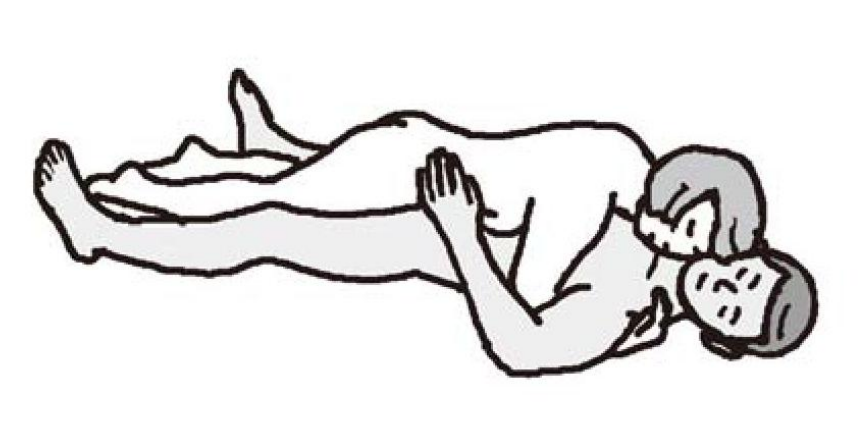
\includegraphics[width=0.7\linewidth]{tw1}
	\caption{}
	\label{fig:1}
\end{figure}

骑乘位若是容易射精,可改为抱住女方,让两人身体贴紧,女方双腿置于男方双腿之间。为了缓和,进行深呼吸。两人的接触面积大,因此能够产生安心感。

\subsection{挺背深呼吸的正常位}

正常位容易射精,是因为前倾姿势使得兴奋时的交感神经占优势,所以要挺直背脊,一边深呼吸,一边看着女方的表情,享受缓缓抽插的乐趣。

\begin{figure}[htbp]
	\centering
	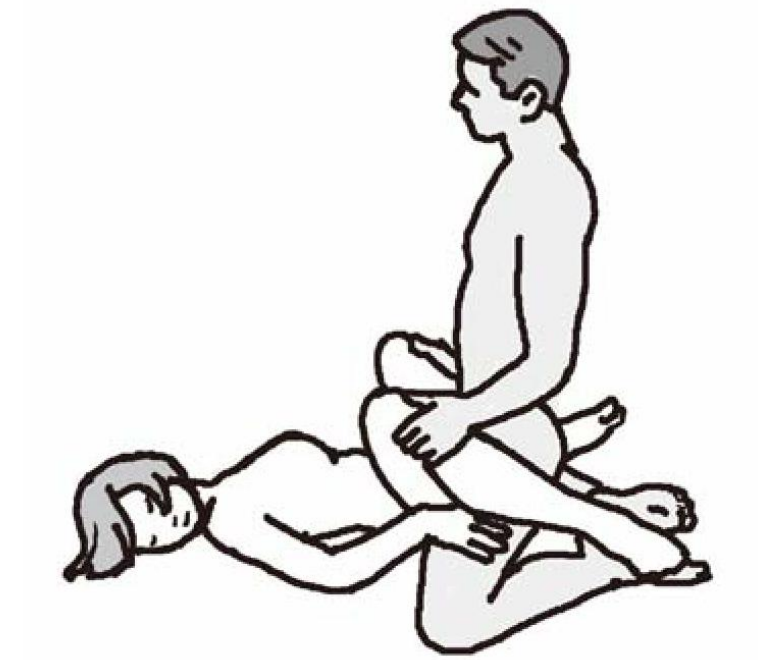
\includegraphics[width=0.7\linewidth]{tw2}
	\caption{}
	\label{fig:1}
\end{figure}

\subsection{松葉式}

女方仰躺,男方以横躺的姿势插入。女方单腿跨在男方肩上,两人身体有如交错的松叶般交缠。男方的手可以同时爱抚女方的胸部或阴蒂。由于腰部无法过度扭动,反而能够充分享受缓缓抽插的乐趣。

\begin{figure}[htbp]
	\centering
	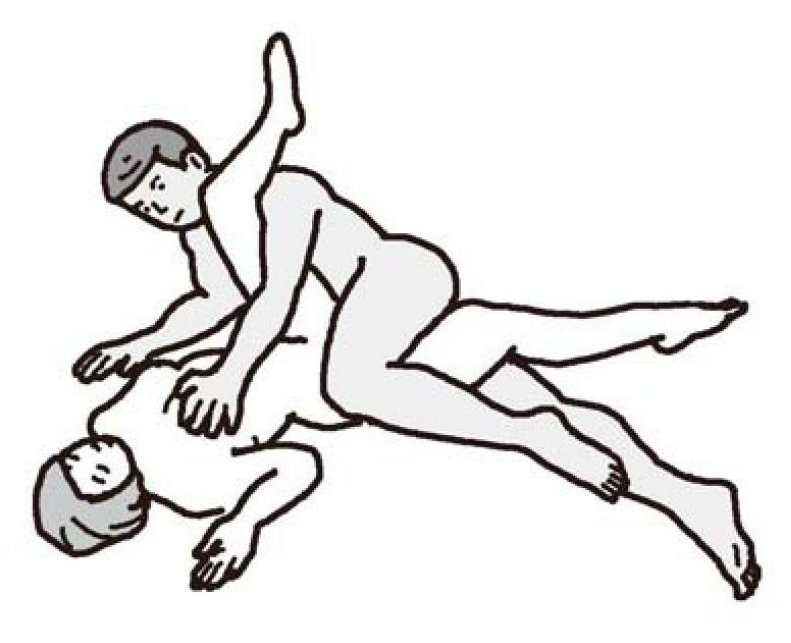
\includegraphics[width=0.7\linewidth]{tw3}
	\caption{}
	\label{fig:1}
\end{figure}

\subsection{深擁的正常位}

正常位容易射精,因此感觉到快要射精时,暂时停止腰部扭动,抱紧女方,让两人身体紧贴,稍微休息片刻,一边亲吻对方,一面等待情绪逐渐缓和。

\begin{figure}[htbp]
	\centering
	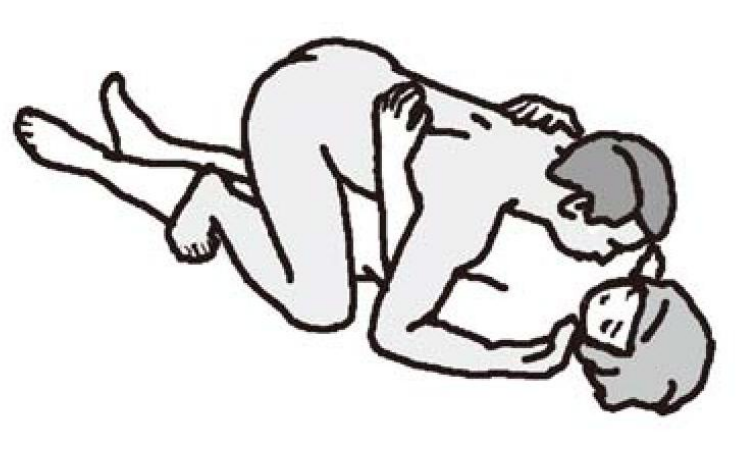
\includegraphics[width=0.7\linewidth]{tw4}
	\caption{}
	\label{fig:1}
\end{figure}

\section{让容易阳痿的男人持久的体位}

避免爱爱中途阴茎突然软掉的“阳痿”窘况。为了英挺持久,不妨采取刺激视觉又能紧贴阴茎的体位。

\subsection{M字腿骑乘位}

女方双腿打开呈M字的骑乘位变化式。由于女方的腿大幅张开,故两人交合的部位能够一览无遗,给予视觉强烈的刺激。女方背向男方的话,则容易刺激G点。

男方可以单手爱抚女方阴蒂,快感能使阴道紧缩。

\begin{figure}[htbp]
	\centering
	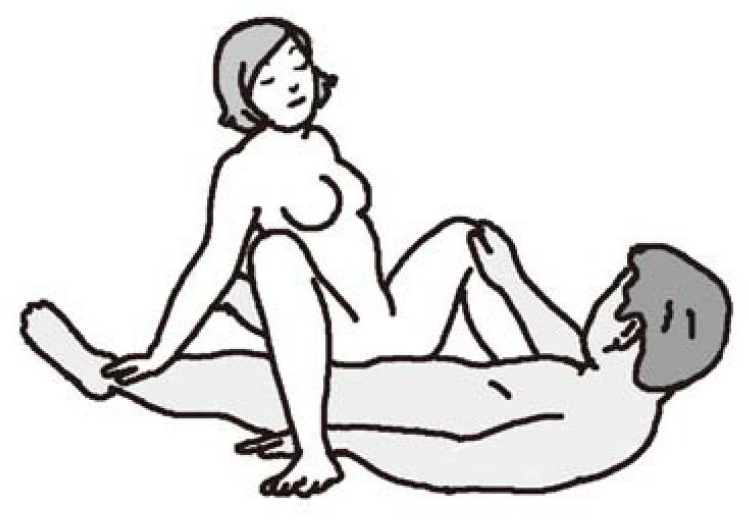
\includegraphics[width=0.7\linewidth]{tw5}
	\caption{}
	\label{fig:1}
\end{figure}

\subsection{反转松葉式}

女方上半身侧躺,男方抬起女方单腿,由侧面插入。介于正常位与背向位之间插入,便不会因为变换体位而使阴茎“鬆脱”,能够防止中途软掉。

\begin{figure}[htbp]
	\centering
	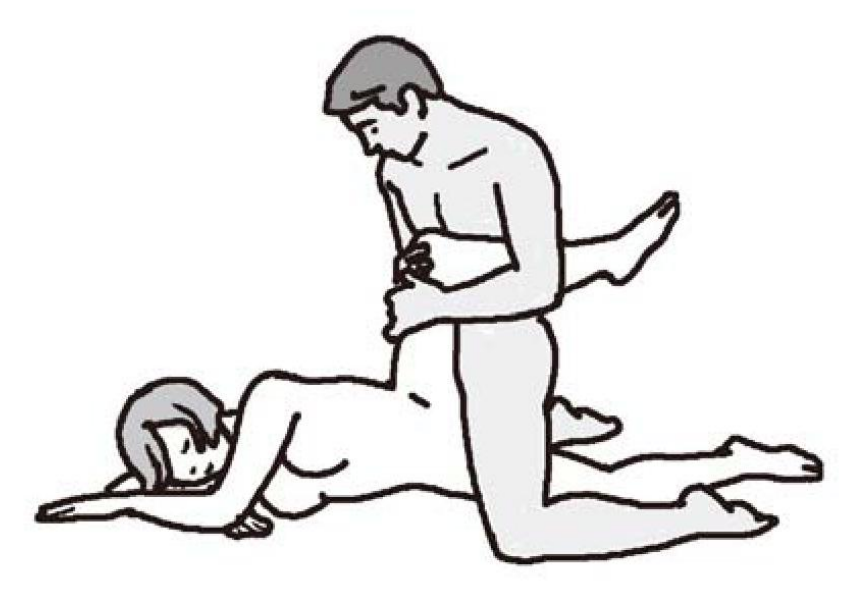
\includegraphics[width=0.7\linewidth]{tw6}
	\caption{}
	\label{fig:1}
\end{figure}

\subsection{不倒翁}

女方双腿并拢,身体微微弓起。男方抱着女方膝盖,往女方胸部方向前倾,以跪姿深深插入。这是男性腰部容易摆动的体位。女方可以藉由膝盖的开合调整两人交合的紧密程度。

\begin{figure}[htbp]
	\centering
	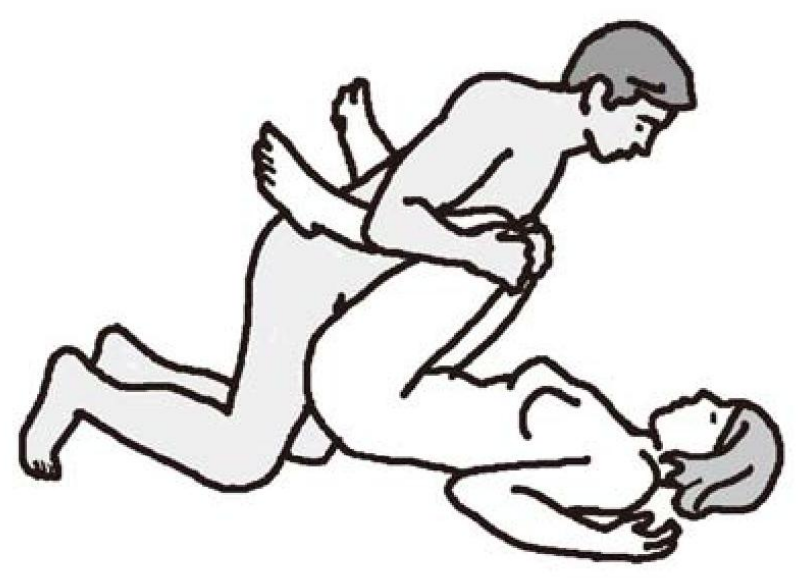
\includegraphics[width=0.7\linewidth]{tw7}
	\caption{}
	\label{fig:1}
\end{figure}

\subsection{三点进攻的背向位}

就算阴茎中途突然软掉,也绝对不要焦虑。男方可以从女方背后一边抽插,一边爱抚阴蒂与胸部,便能若无其事地掩饰中途不举的状况,同时增加女方的快感。

\begin{figure}[htbp]
	\centering
	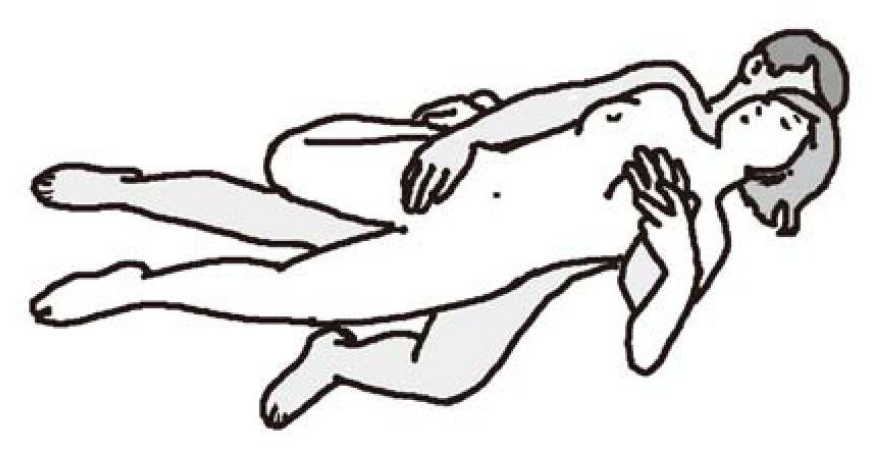
\includegraphics[width=0.7\linewidth]{tw8}
	\caption{}
	\label{fig:1}
\end{figure}

\section{预防腰痛的体位}

爱爱中途突然闪到腰,是让人感叹上了年纪的瞬间。为了减少男人腰部的负担,建议采取预防腰痛的体位。

\subsection{颜面坐姿式}

男方盘腿坐着,女方跨坐在上面。男方不要用腰部前后扭动,而是利用膝盖上下摆动。如果能利用弹簧床借力使力,更能减轻腰部负担。

\begin{figure}[htbp]
	\centering
	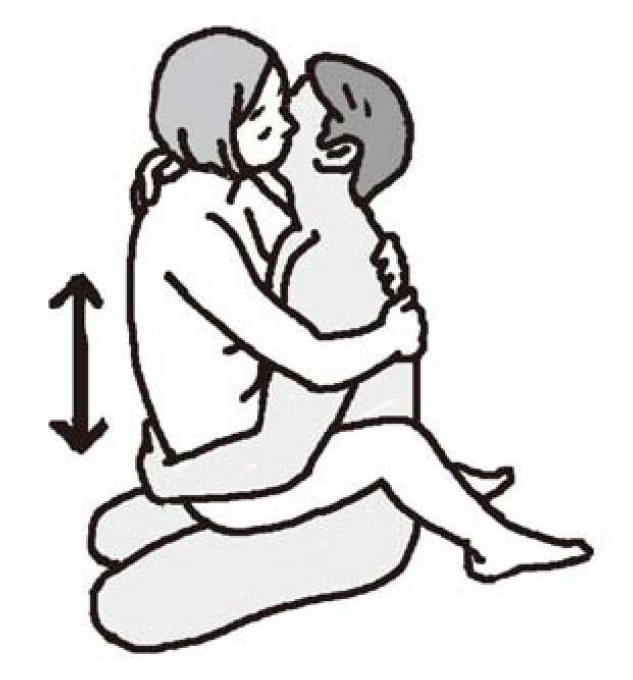
\includegraphics[width=0.7\linewidth]{tw9}
	\caption{}
	\label{fig:1}
\end{figure}

\subsection{曲膝骑乘位}

两人以筏茶臼式交合后,男方单脚屈膝,或是双脚都屈膝,有如要弹起女伴般扭动腰部。由于膝盖弯曲,因此比较容易摆动。

\begin{figure}[htbp]
	\centering
	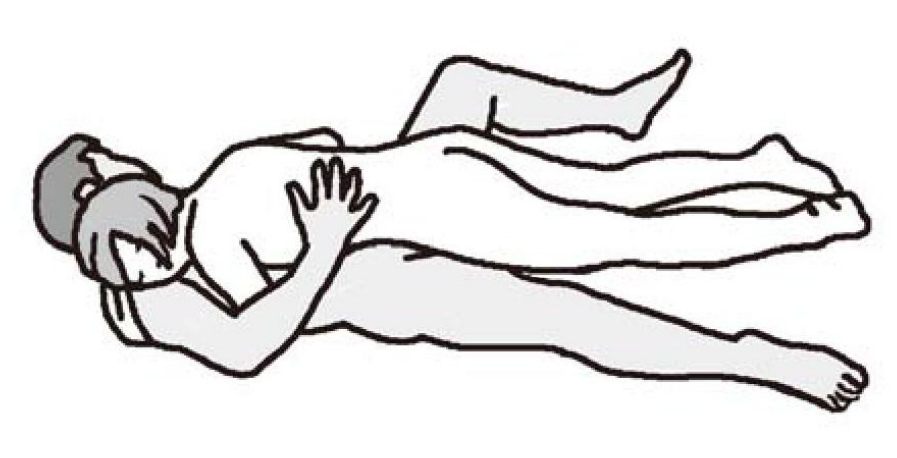
\includegraphics[width=0.7\linewidth]{tw10}
	\caption{}
	\label{fig:1}
\end{figure}

\subsection{下腰后趴位}

男方以蹲姿打开双膝,双手向后伸直支撑上半身,腰部前挺以稳定姿势。女方背向男方采趴姿跪在男方双腿之间。男方协助女方前后扭动。

\begin{figure}[htbp]
	\centering
	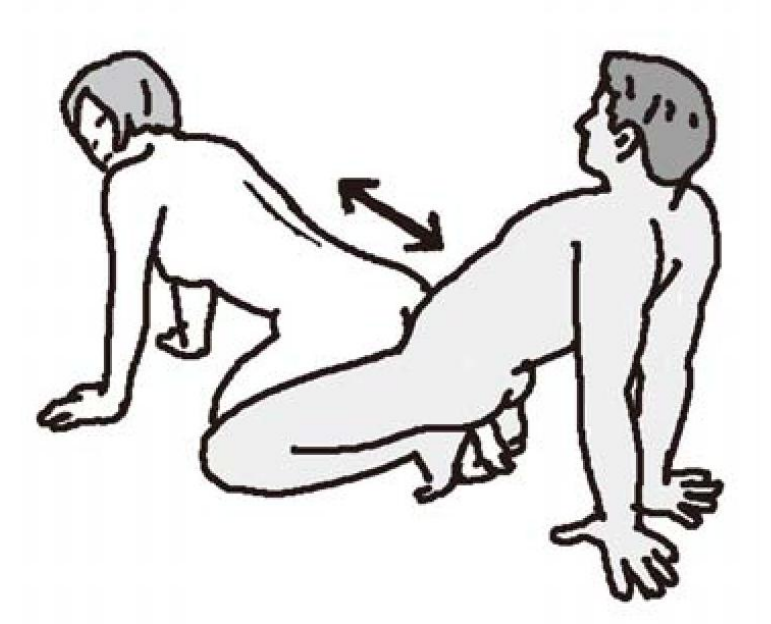
\includegraphics[width=0.7\linewidth]{tw11}
	\caption{}
	\label{fig:1}
\end{figure}

\subsection{弯腰背向位}

利用床或沙发的站立背向位。女方向前弯腰,双手撑住床沿或沙发,男方由后方插入。男方双手扶住女方腰部以稳定姿势,只需前后摆动,几乎不会对男方的腰部造成负担。

\begin{figure}[htbp]
	\centering
	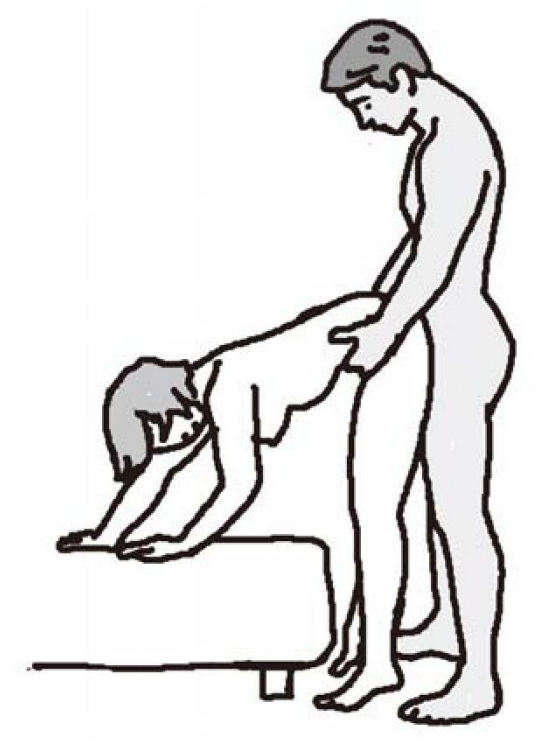
\includegraphics[width=0.7\linewidth]{tw12}
	\caption{}
	\label{fig:1}
\end{figure}

\section{传达满满爱意的体位}

能够传递满满爱意的体位,关键在于:

十指交扣等紧密接触

容易亲吻对方

长时间交合

凝视双眼,说出爱语,身体会从最深处开始融化。

\subsection{织茶臼}

两人以骑乘位姿势十指交扣。女方在激烈的云雨时,不会失去身体平衡,而且能够轻松地摆动腰部。两人还可以透过双手交缠感受彼此的爱意。

\begin{figure}[htbp]
	\centering
	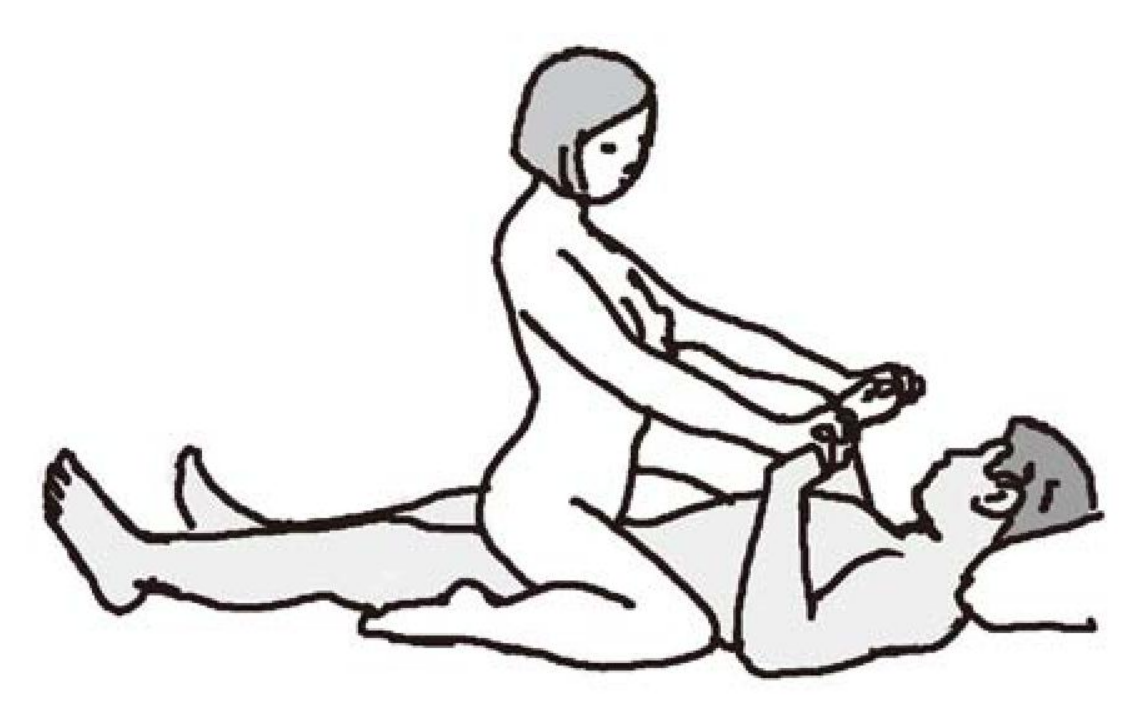
\includegraphics[width=0.7\linewidth]{tw13}
	\caption{}
	\label{fig:1}
\end{figure}

\subsection{彩虹桥}

\begin{figure}[htbp]
	\centering
	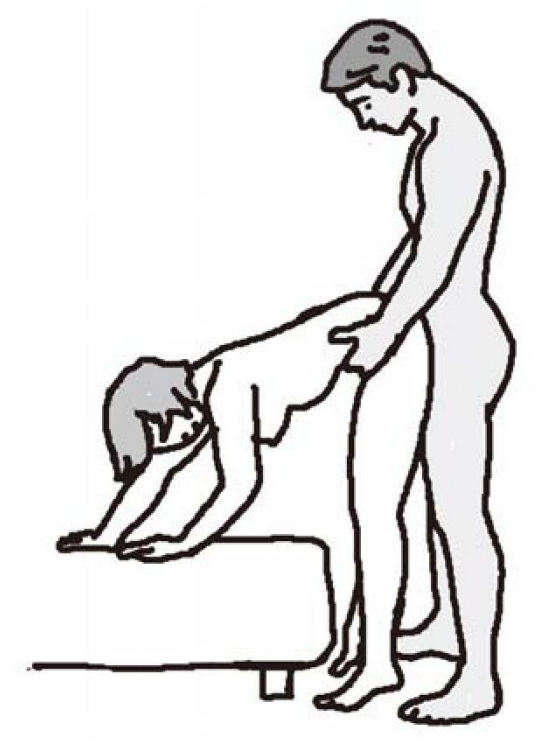
\includegraphics[width=0.7\linewidth]{tw12}
	\caption{}
	\label{fig:1}
\end{figure}

\subsection{}

\begin{figure}[htbp]
	\centering
	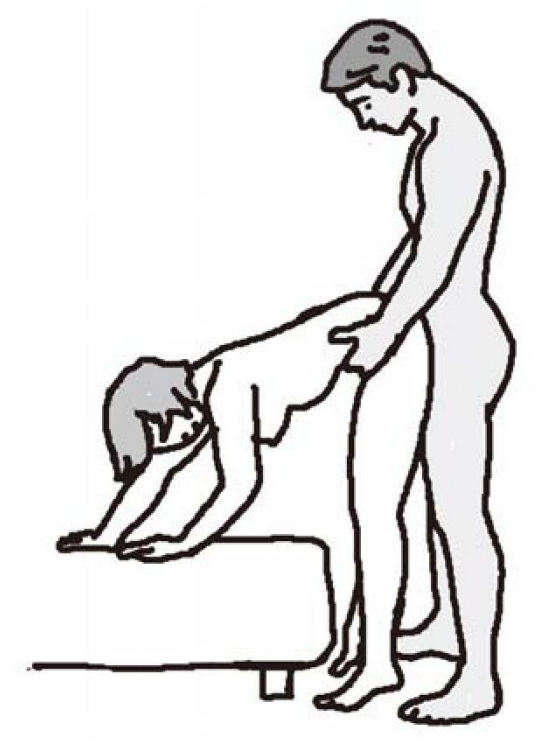
\includegraphics[width=0.7\linewidth]{tw12}
	\caption{}
	\label{fig:1}
\end{figure}

\subsection{}

\begin{figure}[htbp]
	\centering
	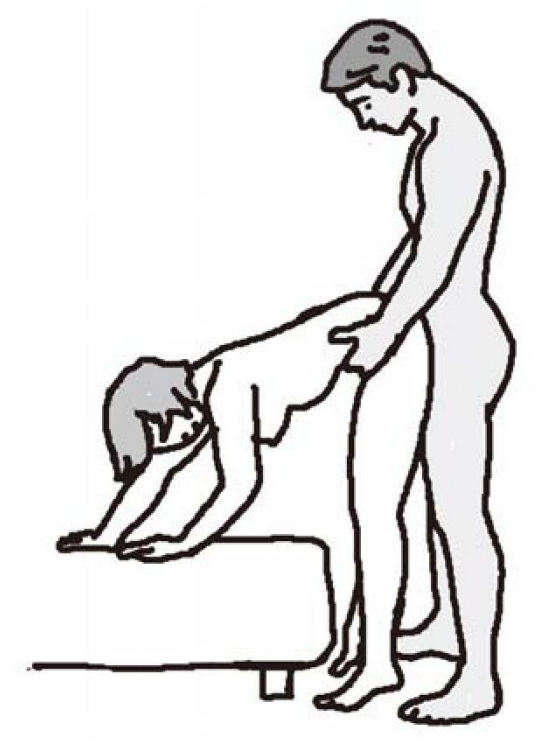
\includegraphics[width=0.7\linewidth]{tw12}
	\caption{}
	\label{fig:1}
\end{figure}

\subsection{}

\begin{figure}[htbp]
	\centering
	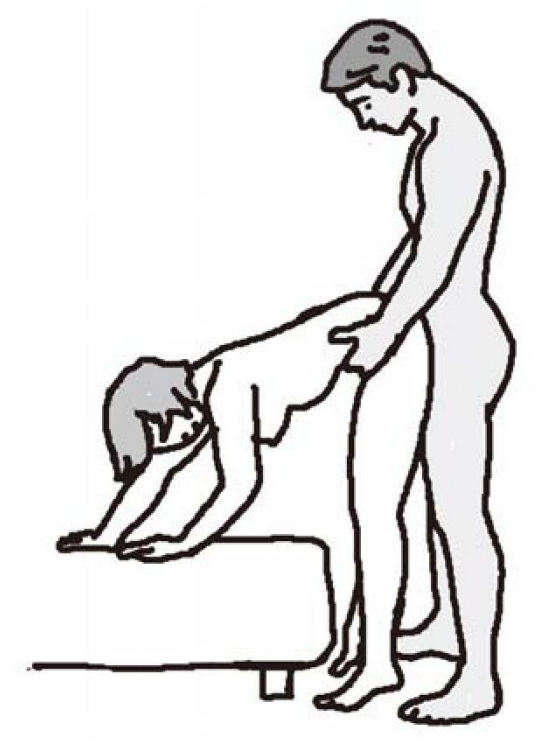
\includegraphics[width=0.7\linewidth]{tw12}
	\caption{}
	\label{fig:1}
\end{figure}

\subsection{}

\begin{figure}[htbp]
	\centering
	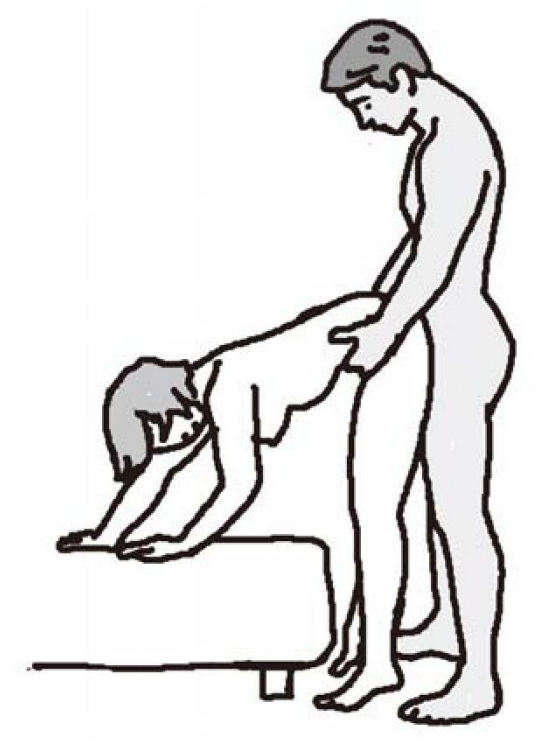
\includegraphics[width=0.7\linewidth]{tw12}
	\caption{}
	\label{fig:1}
\end{figure}\subsection{}

\begin{figure}[htbp]
\centering
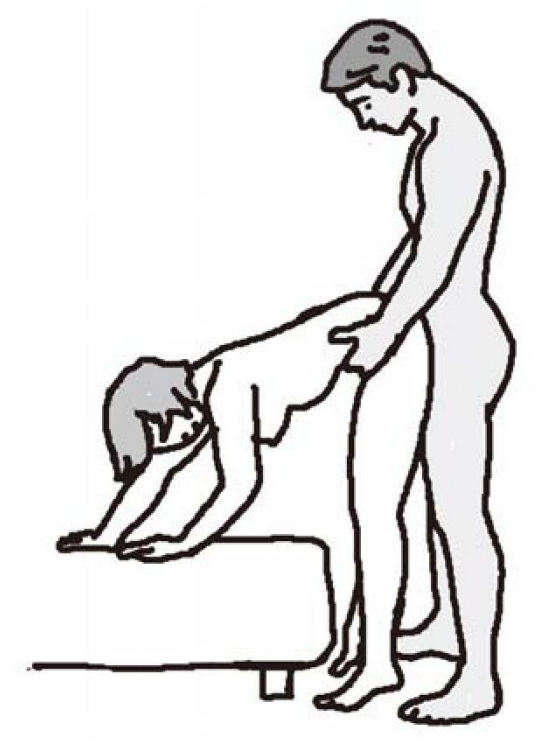
\includegraphics[width=0.7\linewidth]{tw12}
\caption{}
\label{fig:1}
\end{figure}\subsection{}

\begin{figure}[htbp]
\centering
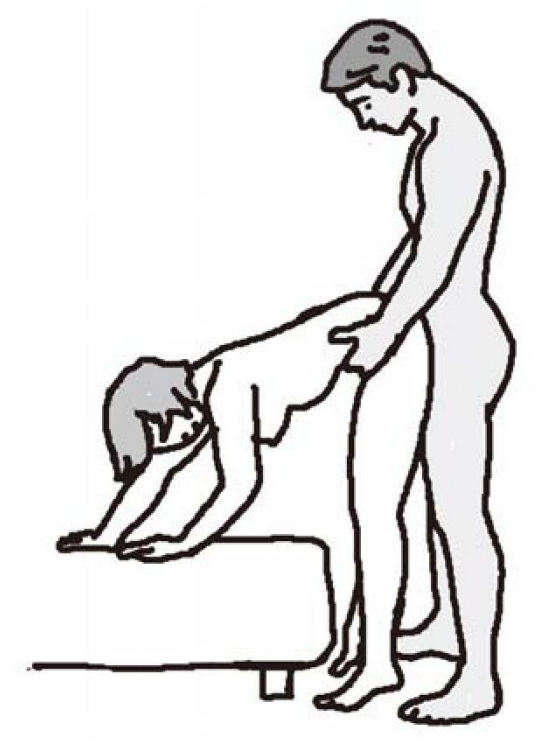
\includegraphics[width=0.7\linewidth]{tw12}
\caption{}
\label{fig:1}
\end{figure}\subsection{}

\begin{figure}[htbp]
\centering
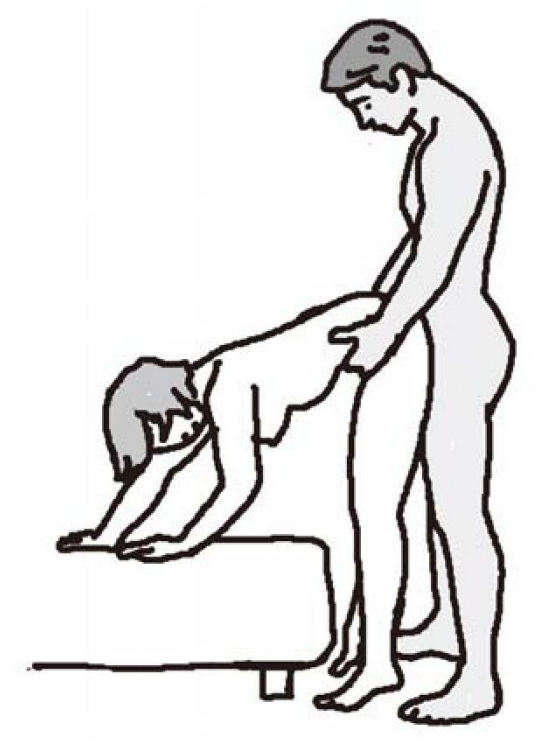
\includegraphics[width=0.7\linewidth]{tw12}
\caption{}
\label{fig:1}
\end{figure}\subsection{}

\begin{figure}[htbp]
\centering
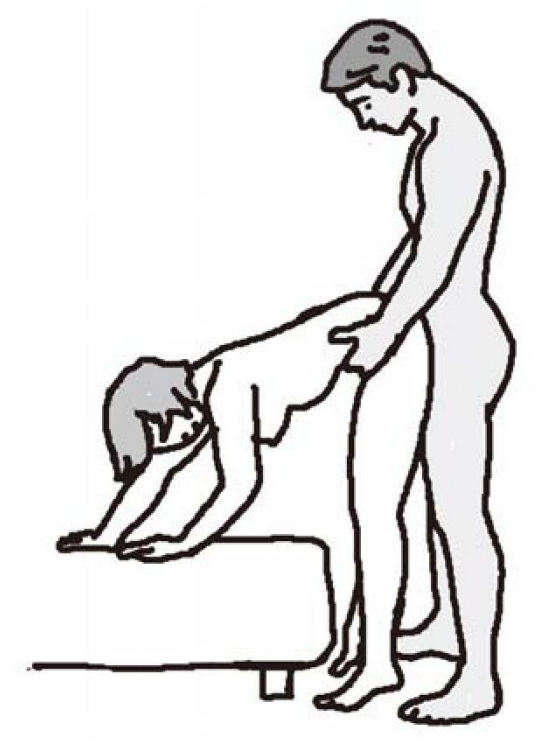
\includegraphics[width=0.7\linewidth]{tw12}
\caption{}
\label{fig:1}
\end{figure}\subsection{}

\begin{figure}[htbp]
\centering
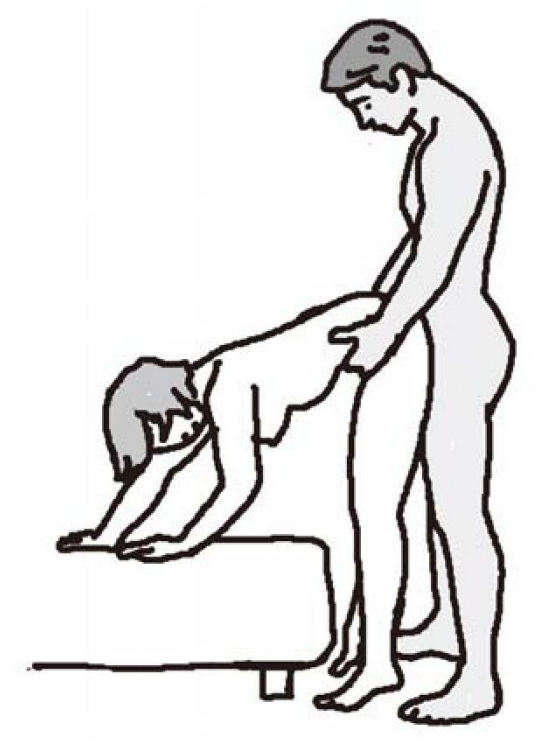
\includegraphics[width=0.7\linewidth]{tw12}
\caption{}
\label{fig:1}
\end{figure}\subsection{}

\begin{figure}[htbp]
\centering
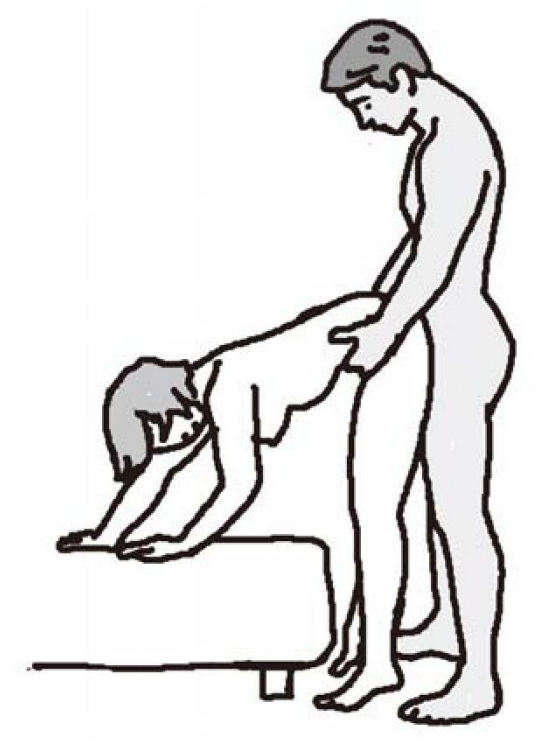
\includegraphics[width=0.7\linewidth]{tw12}
\caption{}
\label{fig:1}
\end{figure}\subsection{}

\begin{figure}[htbp]
\centering
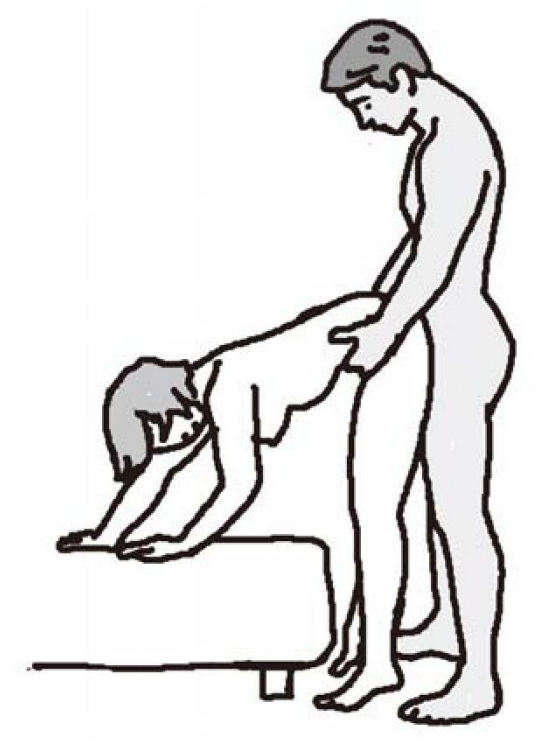
\includegraphics[width=0.7\linewidth]{tw12}
\caption{}
\label{fig:1}
\end{figure}\subsection{}

\begin{figure}[htbp]
\centering
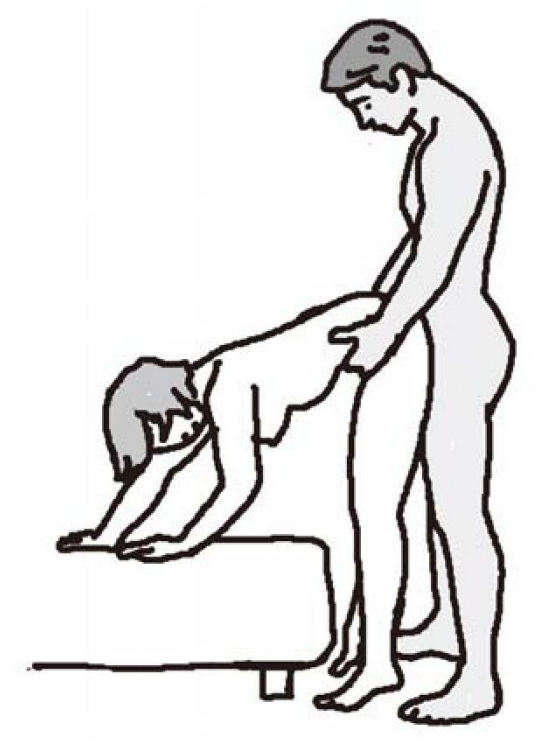
\includegraphics[width=0.7\linewidth]{tw12}
\caption{}
\label{fig:1}
\end{figure}\subsection{}

\begin{figure}[htbp]
\centering
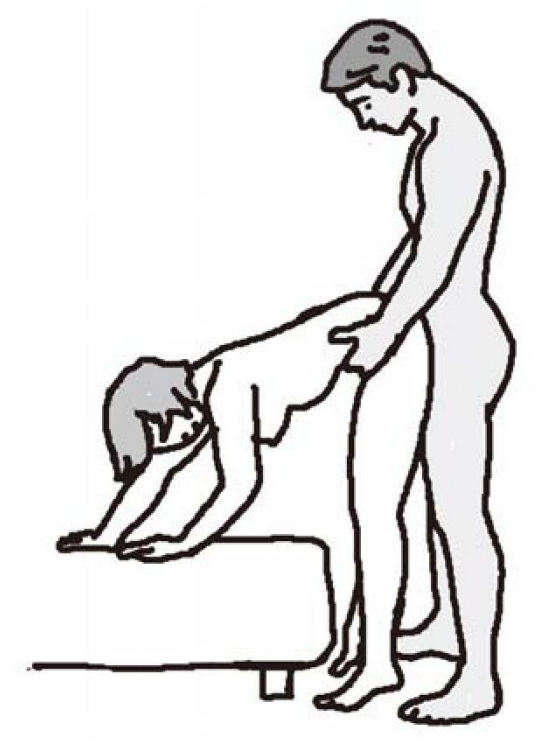
\includegraphics[width=0.7\linewidth]{tw12}
\caption{}
\label{fig:1}
\end{figure}\subsection{}

\begin{figure}[htbp]
\centering
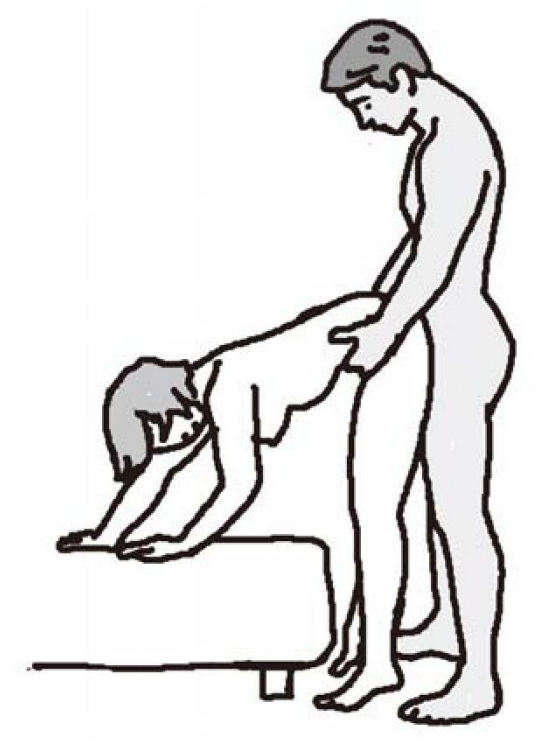
\includegraphics[width=0.7\linewidth]{tw12}
\caption{}
\label{fig:1}
\end{figure}\subsection{}

\begin{figure}[htbp]
\centering
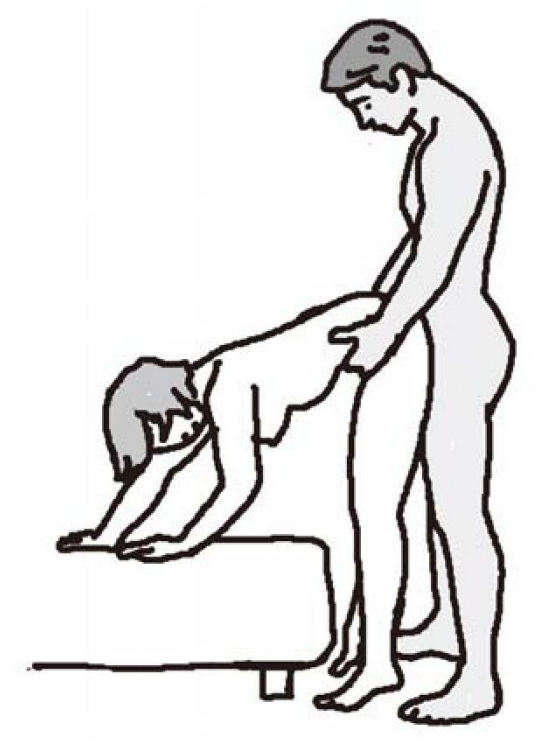
\includegraphics[width=0.7\linewidth]{tw12}
\caption{}
\label{fig:1}
\end{figure}\subsection{}

\begin{figure}[htbp]
\centering
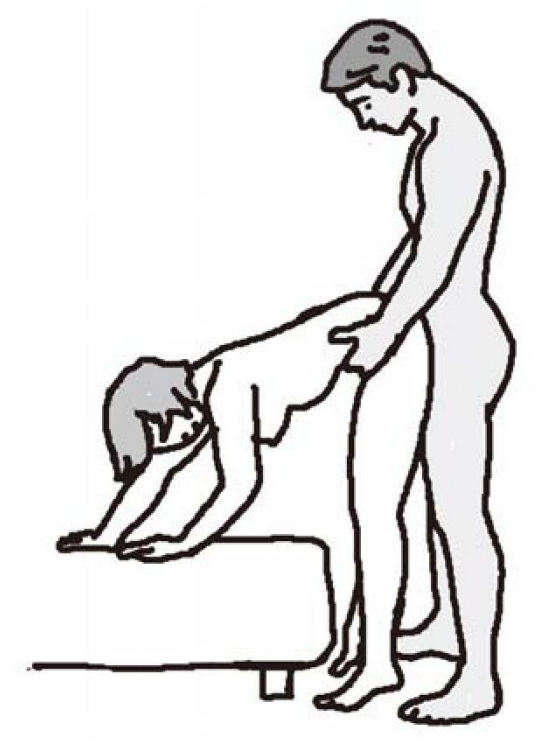
\includegraphics[width=0.7\linewidth]{tw12}
\caption{}
\label{fig:1}
\end{figure}\subsection{}

\begin{figure}[htbp]
\centering
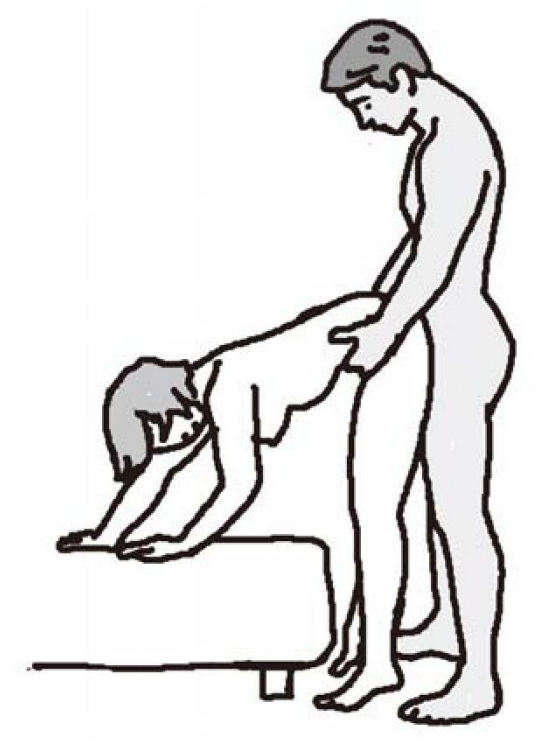
\includegraphics[width=0.7\linewidth]{tw12}
\caption{}
\label{fig:1}
\end{figure}\subsection{}

\begin{figure}[htbp]
\centering
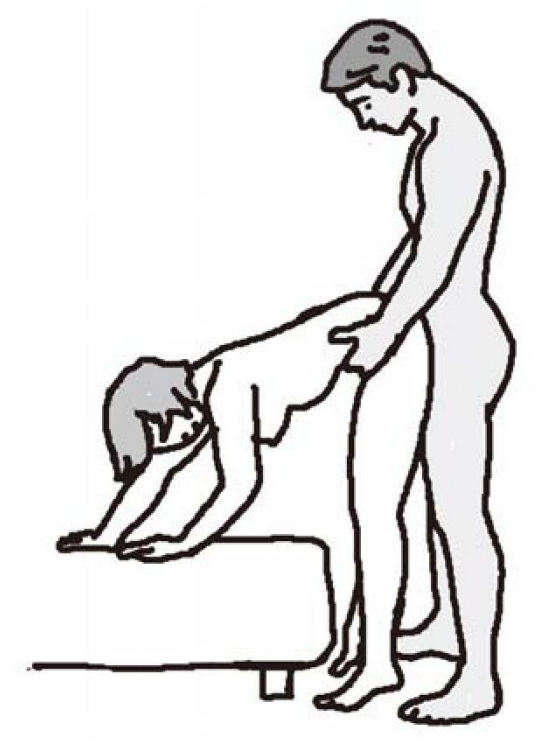
\includegraphics[width=0.7\linewidth]{tw12}
\caption{}
\label{fig:1}
\end{figure}\subsection{}

\begin{figure}[htbp]
\centering
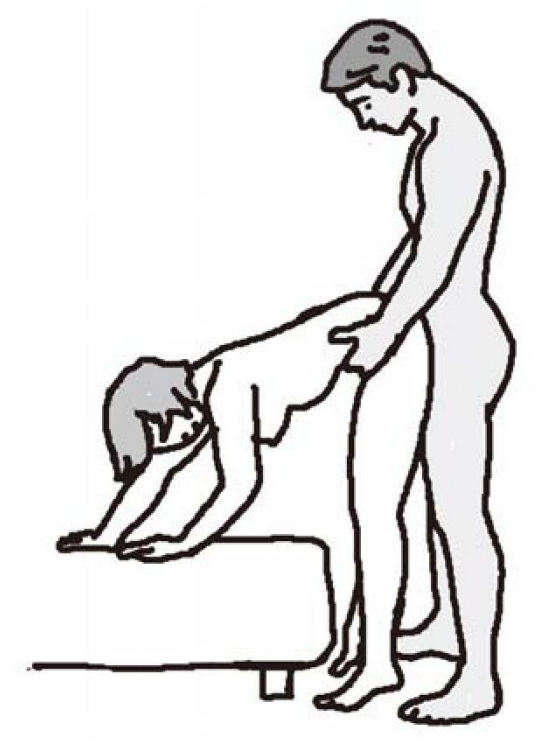
\includegraphics[width=0.7\linewidth]{tw12}
\caption{}
\label{fig:1}
\end{figure}\subsection{}

\begin{figure}[htbp]
\centering
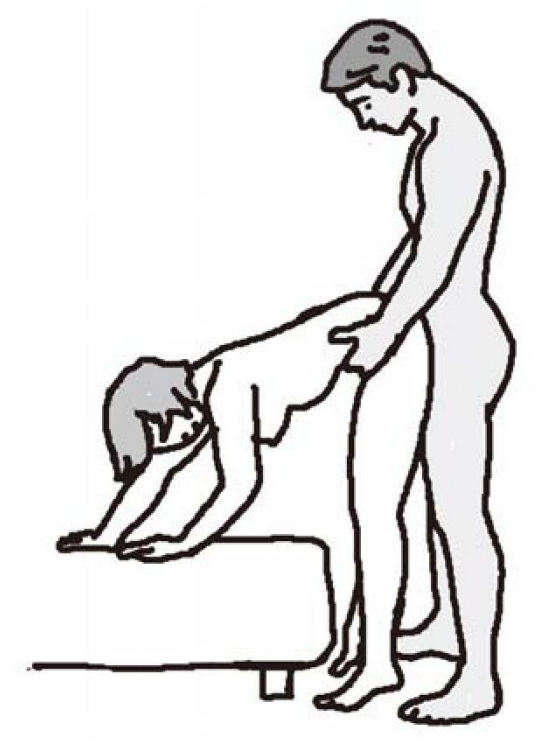
\includegraphics[width=0.7\linewidth]{tw12}
\caption{}
\label{fig:1}
\end{figure}

\backmatter

一起高潮          喜田直江

\end{document}